%%----------Chapter 3------------------------------------------
\chapter{Rule Languages and Tools}

\hspace{0.3in}This chapter presents the rule languages and semantic tools that are relevant to
this thesis. In Section 3.1, we give a brief introduction to rule languages, 
followed by rule engines in Section 3.2. Finally, we discuss the architecture of OO jDREW in Section 3.3.

\section{Rule Languages}

\hspace{0.3in}Besides its focus on Web ontologies, the Semantic Web has a focus on Web rules because they can express policies, regulations, etc for e-Commerce applications, which increased the need for rule languages over the last few years\footnote{\href{www.ruleml.org}{\url{www.ruleml.org}}}. Some of the rule languages are Semantic Web Rule Language (SWRL), Web Rule Language (WRL), Rule Interchange Format (RIF), and Rule
Markup Language (RuleML). RuleML (XML syntax) and its presentation syntax POSL \cite{HB:05} are the declarative languages that we have used in this thesis.

\subsection{Rule Markup Language}

\hspace{0.3in}The Rule Markup Initiative has defined a shared Rule Markup Language (RuleML), permitting both forward (bottom-up) and backward (top-down) rules in XML for deduction, rewriting, and further inferential-transformational tasks as well as XML-based production and reaction rules for (event-)condition-action tasks. Over the years, rules, as exemplified by RuleML, PRR \cite{DBLP:conf/w3c/TabetWSVJMPFD05}, and RIF \cite{Boley:08:RBL} have shown their impact on e-Commerce as well as the Semantic Web. Moreover, rule interchange is playing a significant role in Knowledge Representation (KR) \cite{HB:01}, as exemplified by Common Logic\footnote{\href{http://cl.tamu.edu}{\url{http://cl.tamu.edu}}}.

\hspace{0.3in}RuleML is built using input from other standards work, i.e.,  Mathematical Markup Language (MathML),
DARPA Agent Markup Language (DAML), and Extensible Stylesheet Language Transformations (XSLT) as well as co-evolving with the above-mentioned efforts that allows to publish and share rulebases on the World Wide Web. The goal of RuleML is put forward in a Coverpages technology report \cite{Tech:06}.

\begin{quote}
    ``Our main goal is to provide a basis for an integrated rule-markup
    approach that will be beneficial to all involved and to the rule
    community at large ... This RuleML kernel language can serve as a
    specification for immediate rule interchange and can be gradually
    extended ... "
\end{quote}

\hspace{0.3in}RuleML 0.91 is the current version sustaining a family of sublanguages, such as First Order Logic (FOL)
RuleML, SCLP RuleML (Situated Courteous Logic Programs RuleML), Fuzzy RuleML, and Reaction RuleML. In this thesis, we focus only on (Object Oriented)RuleML, an extension of RuleML, now part of RuleML 0.91, that permits ``slotted" (attribute-value) typed descriptions in RuleML.

\subsection{Positional-Slotted Language}

\hspace{0.3in}Prolog, which stands for PROgramming in LOGic \cite{CM:04}, is the most widely available language in the logic programming paradigm. It is based on the  mathematical notions of relations and logical inference. Prolog is a logic programming language that uses the Horn subset of first order logic.

\hspace{0.3in}Prolog is a declarative language whose Horn clauses can be facts as well as rules used to describe problems rather than coding algorithms as in the imperative programming. Prolog allows the user to issue a query, and its engine searches and applies clauses in order to provide the user with an answer.

\hspace{0.3in}POSL is derived from Prolog. It is a human-readable (presentation) syntax for Semantic Web knowledge. It combines Prolog's positional and F-logic's (standing for Frame Logic) \cite{MK:95} slotted syntaxes for representing knowledge (facts and rules) in the Semantic Web. In \cite{HB:05}, the author describes that POSL not only accommodates many kinds of assertional-logical and object-centered modeling styles, but also achieves conciseness and orthogonality at large. The compactness of the language makes it easier for humans to write and read in POSL than in XML syntax.
Since it is interconvertible with RuleML, the advantage of XML, being more machine-readable, is thus preserved. The bidirectional translator for POSL to RuleML and vice-versa is available online\footnote{\href{http://www.jdrew.org/oojdrew}{\url{www.jdrew.org/oojdrew}}}.

\section{Adaptation of the Rule Engine OO jDREW}

\hspace{0.3in}In this section, we describe the rule engine OO jDREW, which serves as a tool for RuleML. Mandarax \cite{md:05}, SweetRules \cite{sr:05} and jDREW \cite{JD:05} have also been developed as rule engines supporting various subsets of RuleML.

\subsection{Basic OO jDREW}

\hspace{0.3in}OO jDREW is an object oriented extension of jDREW (java Deductive Reasoning Engine for the Web) \cite{JD:05}. It is a reasoning engine for executing RuleML rule markup and the Object Oriented extension for RuleML as well. OO jDREW is one of the engines used by the distributed Rule Responder architecture\footnote{\href{http://responder.ruleml.org}{\url{http://responder.ruleml.org}}}.

\hspace{0.3in}OO jDREW has two modes of operations: OO jDREW
BU (Bottom Up) and OO jDREW TD (Top Down). Bottom-up execution (forward reasoning) is used to infer all derivable knowledge from a set of clauses. Such bottom-up reasoning uses as input facts at the bottom of a proof tree while all derivable ones are added as output. 
\hspace{0.3in}Top-down execution (backward reasoning), in contrast, is used to reduce queries from the top-level queries to more specific queries, etc until it may finally succeed with facts unifying with all subqueries.

%\hspace{0.3in} Bottom up reasoning, in the sense of forward reasoning, resolves a fact against a premise of
%a rule. The visualization of bottom up reasoning shows the input facts at the bottom of the tree while the derived ones are seen at
%the top. In contrast, top down reasoning, namely backward reasoning, is used to resolve a problem from the more general to the more specific and finally reaches the exact query of the reasoning.

\begin{description}
  \item[OO jDREW BU:] In OO jDREW Bottom Up, rules are used to derive new facts
from given facts until a fix point is reached. Three features are
designed in OO jDREW BU: 
\begin{itemize}
\item Type Definition, realized in RDFS and POSL syntax, which comprises the subClassOf taxonomy (type hierarchy for the user's KB
\item Assertional KB, permitting both RuleML and POSL syntax, stores the facts and rules used for Bottom up deduction
\item Running the Forward Reasoner, either in RuleML or POSL syntax, provides users with all derived facts and 
after executing the forward reasoning.
\end{itemize}
\end{description}

\begin{description}
\item[OO jDREW TD:] In OO jDREW Top Down, rules are used to answer queries by
reducing them to subqueries until facts are reached.
Three features are designed in OO jDREW TD: 
\begin{itemize}
\item Type Definition, which is same as in OO jDREW BU 
\item KB, which stores the fact and rules, as in OO jDREW BU, for query on demand
\item Querying the KB, either in RuleML or POSL syntax
\end{itemize}
\end{description}


\subsection{Various Architectures of OO jDREW}

\hspace{0.3in}We have experimented with the various models of using the two OO jDREW reasoners (Top-down and Bottom-up). In this section, we will discuss our approaches and issues. We chose one architecture after several rounds of testing of a sample KB for the different architecture modes.

\subsubsection{ Integration of OO jDREW BU and TD}

\hspace{0.3in}We attempted to integrate the two approaches such that our system would work with two levels of computation. We first execute the Bottom-up reasoner and generate derived facts from the original set of clauses. The new KB is then queried as the KB for Top-down execution of OO jDREW.
 
The need for an integrated archtecture comprising Top-down and Bottom-up arose for the shortest path distance computation. We wanted to get precomputed facts from a set of clauses using Bottom-up and then apply some optimization rules on the generated KB to derive the solutions to a user's query. From our experiments we discovered that same set of clauses cannot be always used for both Top-down and Bottom-up OO jDREW.

\hspace{0.3in}The current differences between OO jDREW Top-down and Bottom-up are:
\begin{itemize}
\item Naf (Negation as failure) of OO jDREW TD cannot be used in OO jDREW BU
\item There are variable binding issues in BU with recursive predicates that work well in OO jDREW TD
\end{itemize}

\hspace{0.3in}With these differences, we could not run the KB unchanged in Bottom-up that works well in Top-down execution mode.


\subsubsection{Top-Down FindAll Solutions}

\begin{figure}
\begin{center}
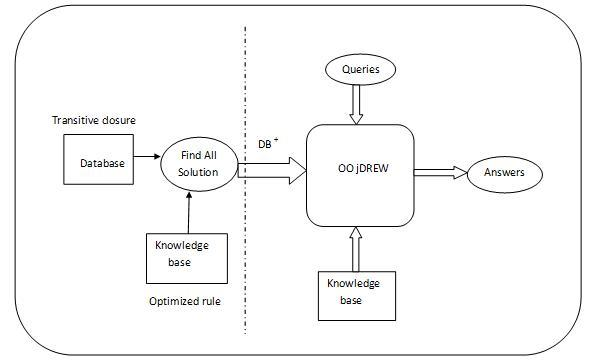
\includegraphics[width=14.8cm, height=6.5cm]{figure1}
\caption {Top-Down FindAll Solutions}
\label{fig:Fig1.1}
\end{center}
\end{figure} 

\hspace{0.3in} After testing a sample KB in both modes of execution, we decided to primarily use Top-down execution for almost all rulebases in our KB. To permit this, the backward reasoning engine has been internally enhanced with a primitive to find all solutions to a query collecting all solutions that would normally be delivered one at a time. The Top-Down FindAll Solutions primitive allows the Top-down engine to first find all (of finitely many) solutions to a selected query. The answer is then returned as a fact base of the primitive parameterized by the query. The architecture of Top-Down FindAll Solutions in OO jDREW is as shown in Figure 3.1. We use this architecture to solve the problem of optimal distance computation in terms of shortest route time. The distanceTime facts and the transitive closure dTR predicates will be stored in the database. Our Findall Solutions class generates all possible routes between every pair of provinces. We then apply the optimization rule to find the shortest route between every pair from the generated dTR facts. Our new database of precomputed route facts will be added to the main KB and used in the TD backward reasoner to answer various queries.

%The TD Find all solution is similar to ``tupOf" function in Functional logic programming and ``univ" in Prolog.



